\chapter{Vergleich von 4G EPS-AKA und 5G-AKA}
\label{chap:3}

Das 4G EPS-AKA Protokoll ist Teil des 4G Standards, dem Vorgänger des 5G Standards, zu dem das 5G-AKA Protokoll gehört.
Beide Protokolle sind \textit{Authentication and Key Agreement} Protokolle und haben somit einiges an Gemeinsamkeiten, sie unterscheiden sich aber auch voneinander.
% Hier beschreiben, dass die Infos nicht aus der Spezfikation stammen sondern aus dem 'Comparative Introduction' paper.

\section{Beschreibung des 4G EPS-AKA Protokolls}

Das 4G EPS-AKA Protokoll ist eines von mehreren Protokollen des 4G Standards.
Es ist für den Austausch eines Schlüssels zur weiteren Kommunikation zuständig.

Die Entitäten des 4G EPS-AKA Protokolls lassen sich in die drei Teile \textit{User Equipment}, \textit{Serving Network} und \textit{Home Network} unterteilen.
Das \gls{ue} ist das \textit{User Equipment} und stellt die Komponenten dar, die sich bei dem Benutzer befinden, z.B. im Smartphone.
Die \gls{enodeb} und die \gls{mme} sind Teil des \textit{Serving Network} und befinden sich bei dem Netzbetreiber, der das Netzwerk dem Benutzer zur Verfügung stellt.
Der \gls{hss} ist Teil des \textit{Home Network} und befindet sich bei dem Netzbetreiber, der dem Benutzer z.B. die SIM-Karte ausgestellt hat. %A Comparative Introduction of 4G and 5G Authentication

\subsection{Ziele}

Ziel des 4G EPS-AKA Protokolls ist es, wie auch beim 5G-AKA Protokoll, den Benutzer und das Netzwerk gegenseitig zu authentifizieren und einen gemeinsamen \textit{''Anchor Key''} bereitzustellen der von nachfolgenden Protokollen verwendet werden kann.
Im Gegensatz zum 5G-AKA Protokoll gibt es beim 4G EPS-AKA Protokoll jedoch Teilnehmer die nicht über den Erfolg der Authentifizierung Bescheid wissen.
Aus dem \textit{''Anchor Key''} können ebenfalls weitere Schlüssel für unterschiedliche Verwendung abgeleitet werden.
Eine Übersicht über die ableitbaren Schlüssel ist in Abbildung 6.2-1 und 6.2-2 des 3GPP TS 33.401 V15.4.0 zu finden. % 3GPP TS 33.401 V15.4.0 Page 33 & 35

\subsection{Das Protokoll}

\begin{figure}[H]
  \centering
  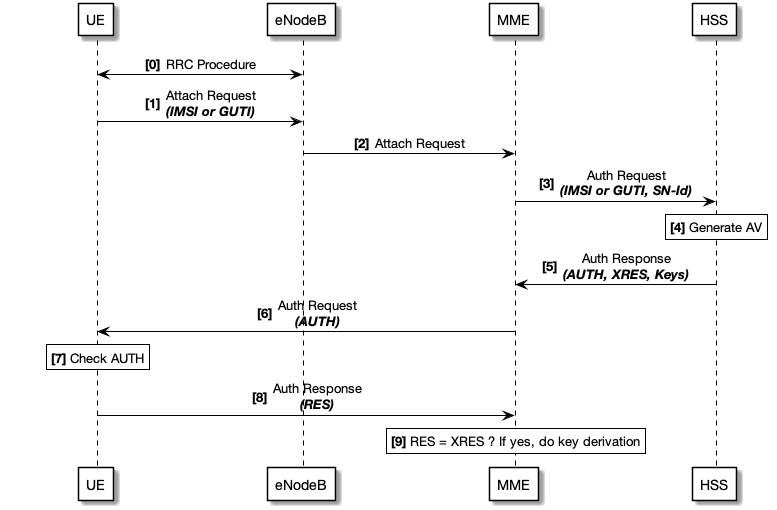
\includegraphics[width=\textwidth]{uml/4g-protocol_v1.png}
  \caption{Das 4G EPS-AKA Protokoll}
  \label{fig:4g_protocol_v1}
\end{figure} %A Comparative Introduction of 4G and 5G Authentication

\begin{enumerate}
\setcounter{enumi}{-1}
%0
\item Bevor das 4G EPS-AKA Protokoll mit \textit{Schritt 1} starten kann muss die \gls{rrc} Prozedur zwischen dem \gls{ue} und der \gls{enodeb} erfolgreich abgeschlossen sein.

%1
\item In Schritt 1 schickt das \gls{ue} den \textit{Attach Request} an den \gls{enodeb} und beginnt somit das 4G EPS-AKA Protokoll.
Die Nachricht enthält entweder die \gls{imsi} oder den \gls{guti} und wird durch das erfolgreiche abschließen der \gls{rrc} Prozedur ausgelöst.

%2
\item In Schritt 2 wird der \textit{Attach Request} aus \textit{Schritt 1} von der \gls{enodeb} an die \gls{mme} weitergesendet.

%3
\item In Schritt 3 sendet die \gls{mme} eine \textit{Auth Request} Nachricht an den \gls{hss}.
Sie enthält entweder die \gls{imsi} oder den \gls{guti}, den die \gls{mme} in \textit{Schritt 2} von der \gls{enodeb} in der \textit{Attach Request} Nachricht erhalten hat und zusätzlich noch die \gls{sn-id} des \textit{Serving Network}s zu dem die \gls{mme} gehört.

%4
\item In Schritt 4 wird aus dem geheimen Schlüssel \textit{K}, den sowohl der \gls{hss} wie auch das \gls{ue} kennen, der \gls{av} generiert.
Er beinhaltet unteranderem die \gls{xres}, die später mit der Antwort des \gls{ue}, \gls{res}, verglichen werden soll, den \gls{auth}, den das \gls{ue} für die Berechnung der \gls{res} benötigt und kryptographischen Schlüssel die im weiteren Verlauf benötigt werden.

%5
\item In Schritt 5 wird der in \textit{Schritt 4} generierte \gls{av} mit der \textit{Auth Response} Nachricht an die \gls{mme} gesendet.

%6
\item In Schritt 6 sendet die \gls{mme} einen \textit{Auth Request} direkt an das \gls{ue}.
Er enthält den \gls{auth}, den das \gls{ue} zur Berechnung der \gls{res} benötigt.

%7
\item Nachdem das \gls{ue} den \gls{auth} Parameter aus \textit{Schritt 6} erhalten hat wird er in Schritt 7 überprüft und daraus die \gls{res} berechnet.

%8
\item In Schritt 8 wird die \gls{res}, die in \textit{Schritt 7} berechnet wurde in einer \textit{Auth Response} Nachricht an die \gls{mme} gesendet.

%9
\item Nach Erhalt der \textit{Auth Response} Nachricht wird in Schritt 9 überprüft ob die \gls{res}, die die \gls{mme} in \textit{Schritt 8} erhalten hat, mit der \gls{xres}, die die \gls{mme} in \textit{Schritt 5} erhalten hat, übereinstimmt.
Ist dies der Fall, so wird aus den kryptographischen Schlüsseln, die die \gls{mme} ebenfalls in \textit{Schritt 5} erhalten hat, unteranderem der \gls{k-asme} der \gls{asme} berechnet, der beispielsweise für die Berechnung weiterer Schlüssel nach der erfolgreichen Authentifizierung benötigt wird.%3GPP TS 33.401 Page 19
\end{enumerate}


\section{Unterschiede von 4G EPS-AKA und 5G-AKA}

Das 4G-EPS-AKA Protokoll und das 5G-AKA Protokoll unterscheiden sich in folgenden Aspekten: %A Comparative Introduction of 4G and 5G Authentication

\begin{itemize}
%User Equipment
\item Das \gls{ue} hat sowohl bei 4G-EPS-AKA, wie auch bei 5G-AKA den gleichen Namen und ahnliche Aufgaben.
In beiden Protokollen beginnt bei dem \gls{ue} die Authentifizierung und ist der symmetrischen Langzeitschlüssel \gls{k} gespeichert.

%Serving Network
\item Das \textit{Serving Network} besteht im 4G EPS-AKA Protokoll aus der \gls{mme}. 
Die \gls{enodeb} kann auch als Teil des \textit{Serving Network}s gesehen werden.
Im 5G-AKA Protokoll hingegen besteht das \textit{Serving Network} nur aus der \gls{seaf}.

%Home Network
\item Im 4G EPS-AKA Protokoll besteht das \textit{Home Network} nur aus dem \gls{hss}.
Im 5G-AKA Protokoll hingegen gesteht das \textit{Home Network} aus der \gls{ausf} und aus dem \gls{udm}/\gls{arpf}/\gls{sidf}.

%Trust Model
\item Sowohl im 4G EPS-AKA wie auch im 5G-AKA Protokoll wird für die Authentifizierung der symmetrischer Langzeitschlüssel \gls{k} benötigt.
Er ist beim 4G EPS-AKA Protokoll im \gls{ue} und im \gls{hss} gespeichert.
Beim 5G-AKA Protokoll ist \gls{k} im \gls{ue} und im \gls{udm}/\gls{arpf} gespeichert.

%UE Identity
\item Jedes \gls{ue} hat eine Zeichenfolge, die es eindeutig identifiziert.
Diese ist jedoch bei den beiden Protokollen unterschiedlich.

Beim 4G EPS-AKA Protokoll kann bei der Kommunikation zwischen \gls{ue} und \textit{Serving Network} die \gls{imsi} oder der \gls{guti} und bei der Kommunikation zwischen \textit{Serving Network} und \textit{Home Network} nur die \gls{imsi} verwendet werden um das \gls{ue} eindeutig zu identifizieren.
Beim 5G-AKA Protokoll hingegen kann bei der Kommunikation zwischen \gls{ue} und \textit{Serving Network} der \gls{suci} oder der \gls{5g-guti} und bei der Kommunikation zwischen \textit{Serving Network} und \textit{Home Network} der \gls{suci} oder der \gls{supi} verwendet werden um das \gls{ue} eindeutig zu identifizieren.

Beim 5G-AKA Protokoll wird zwischen \gls{ue} und \textit{Serving Network} die Identität des \gls{ue} nur verschlüsselt, in Form des \gls{suci} oder des \gls{5g-guti} versendet. Beim 4G EPS-AKA Protokoll hingegen wird auch die unverschlüsselte \gls{imsi} zwischen \gls{ue} und \textit{Serving Network} versendet.

%SN Identity
\item Auch das \textit{Serving Network} kann eindeutig identifiziert werden.
Beim 4G EPS-AKA Protokoll wird das \textit{Serving Network} durch die \gls{sn-id} identifiziert.
Beim 5G-AKA Protokoll hingegen wird das \textit{Serving Network} durch den \gls{sn-name} identifiziert.

Die \gls{sn-id} und der \gls{sn-name} unterscheiden sich jedoch nur dadurch dass dem \gls{sn-name} zusätzlich noch ''5G:'' vorangestellt wurde.

%Authentication of UE decided by
\item Die Entscheidung ob die Authentifizierung erfolgreich war wird bei beiden Protokollen unterschiedlich gehandhabt.

Beim 4G EPS-AKA Protokoll entscheidet nur die \gls{mme}, die Teil des \textit{Serving Network}s ist, ob eine Authentifizierung erfolgreich war.
Die Entscheidung wird somit nur innerhalb des \textit{Serving Network}s getroffen.
Das \textit{Home Network} ist nicht an der Entscheidung beteiligt und wird auch nicht über den Ausgang der Authentifizierung informiert.

Beim 5G-AKA Protokoll hingegen entscheiden sowohl die \gls{seaf}, die Teil des \textit{Serving Network}s ist, wie auch die \gls{ausf}, die Teil des \textit{Home Network}s ist, ob die Authentifizierung erfolgreich war.
Die Entscheidung wird somit sowohl vom innerhalb des \textit{Serving Network}s, wie auch innerhalb des \textit{Home Network}s getroffen.
Des Weiteren benachrichtigt die \gls{ausf} auch das \gls{udm} über den Ausgang der Authentifizierung.
\end{itemize}